\documentclass{article}
\usepackage[utf8]{inputenc}
\usepackage[english]{babel}
\usepackage[]{amsthm} %lets us use \begin{proof}
\usepackage[]{amssymb} %gives us the character \varnothing
\usepackage{mathtools}
\renewcommand{\qedsymbol}{\rule{0.7em}{0.7em}}
\usepackage{amsmath}
\usepackage{titlesec} 
\usepackage{float}

\titleformat{\section}[runin]
  {\normalfont\large\bfseries}{\thesection}{1em}{}
\titleformat{\subsection}[runin]
  {\normalfont\normalsize\bfseries}{\thesubsection}{1em}{}
\titleformat{\subsubsection}[runin]
  {\normalfont\normalsize\bfseries}{\thesubsubsection}{1em}{}

\newcommand{\Int}{\int\limits}


\title{Understanding the dynamics of a complex biological network without 
parameter information: Case study on the cell-cycle network 
of fission-yeast (\textit{S.pombe})}
\author{Souvadra Hati (Sr: 15551)}
\date\today
%This information doesn't actually show up on your document unless you use the maketitle command below

\begin{document}
\maketitle %This command prints the title based on information entered above

%Section and subsection automatically number unless you put the asterisk next to them.
% ************************************************************************* %
%                              Introduction                                 %
% ************************************************************************* %
\section*{Introduction:} Understanding and predicting the dynamics of complex 
biochemical networks is one of the fundamental goal of Systems Biology. Although,
even a single cell is way too complex in nature for us to model all its 
biochemical behaviours using our current understanding and compute capacity,
scientists have been successful in modelling some of the biochemical pathways
essentials in every living organism. One of the computationally feasible ways 
to predict the dynamical behaviours of these networks is to numerically solve a bunch of 
coupled Ordinary Differential Equations (ODEs) with appropriate kinetic parameters 
that can be experimentally measured. But that process requires extensive wet-lab
experiments to find out the vast array of biochemical parameters necessary to 
model even modests of the biological pathways, which slows down the process of 
building the models. This has motivated scientists to come up with innovative 
ideas to be able to gain insight into a biochemical pathway without extensive 
knowledge of the parameters involved in it. In this article I am going to discuss
two such ways of modelling a network and show how they can be useful by applying 
them in the cell-cycle pathway of fission-yeast (\textit{S.pombe}).
% ************************************************************************* %
%                             Discrete Method                               %
% ************************************************************************* %
\section*{Discrete Method:}
One of the most simple yet elegant way to model the essentials of a network is
to model it as a graph model with each protein / regulator can be assumed as 
a node and the interaction between those regulators as the edges of the graph.
The edges will only represent the the sign of the relation between those two nodes.
What I mean, is that the node will only take into account of the fact that 
the interaction is activating (+1) or inhibiting (-1). After that, in each 
discrete ieration the state of the the daughter nodes of the initialized nodes 
(can be themselves as well if self-activation or self-inhibition is present)
will be updated as per the update rule mentioned below.

\begin{equation*}
  S_i (t+1) = \begin{cases}
    0, & \text{if } \sum_{j} a_{ij} S_j(t) < \theta_i\\
    1, & \text{if } \sum_{j} a_{ij} S_j(t) > \theta_i\\
    S_i (t), & \text{if } \sum_{j} a_{ij} S_j(t) = \theta_i
    \end{cases}
\end{equation*}
Here, $S_j(t) \in \{0,1\}$ in the binary value assigned to node $j$ at iteration
$t$, which discretely denotes if the protein is present in the system at that 
iteration or not. $a_{ij} = 1$ denotes an activating interaction from node j to 
node i, and similarly $a_{ij}$ denotes an inhibiting edge and $a_{ij} = 0$
denotes no interaction (no edge between those two nodes). $\theta_{ij}$ is a 
threshold of activation of node $i$ which is generally $0$, unless otherwise 
mentioned \cite{boolean_model}.

One interesting aspect of this Boolean modelling is that, we can actually 
start the model iteration using all the possible initial conditions and that 
will be in most cases very much computationally feasible. For example, if our 
network of interest has 7 nodes, then there will be in total $2^7 = 128$, which 
means we can effectively sample the total solution space of the network which 
is absolutely not possible in a continuous scenario.

So, in this manner, without any knowledge of the kinetic parameters in the model
or ever solving any ODE at all, we can gain insight into the dynamics of the model
as I shall discuss using a case study in the later half of the report.
% ************************************************************************* %
%                           Continuous Method                               %
% ************************************************************************* %
\section*{Continuous Method:} Although the discrete method in theory can provide
us a lot of information regarding the network of interest, the harsh reality 
is that no biological system is actually discrete and introducing even moderate
amount of realism requires us to write the ODE of the reaction kinetics and solve 
them numerically to observe the dynamics of the network. But that requires 
access to the set of kinetic parameters that we are trying to avoid in our 
modelling paradigm. 

So, to tackle that exact challenge Huang et al. 2018 \cite{RACIPE} published 
an article on a software that they named ``RACIPE: Random Circuit Perturbation".
It takes, just like the Boolean method, only the topology of the core regulatory
circuit and unbiasly generates an ensemble of mathematical models, each of which 
is characterized by a unique set of kinetic parameters From the ensemble of 
models, we can analyze the robust dynamical properteis of the core circuit via 
downstream statistical analysis. In RACIPE, the effects of the "peripheral 
factors" are modeled as random perturbations to the kinetic parameters. RACIPE
samples its parameters across a wide range (via some random distribution) 
keeping the half functional rule (
which states that each regulatory link has about $50\%$ chance to be activated)
valid. The RACIPE generated gene-expression data can later be analyzed using 
differnt statistical tools (primarily Hierarchical clustering analysis (HCA), 
and Principal Component Analysis (PCA)) to get a holistic view of the dynamical 
feature of the network. All these are based of the previous studies that says 
that robust features in any gene regulatory network remains conserved against
large parameter purturbations due to the the restraints from the circuit 
topology itself. 

\begin{figure}[H]
  \centering
  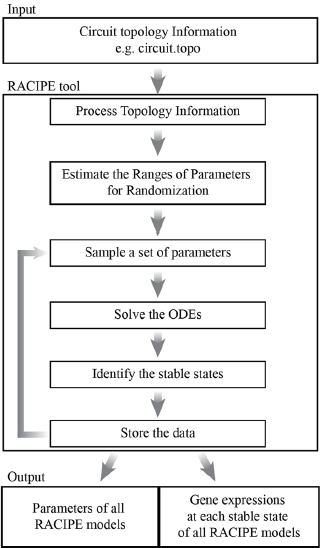
\includegraphics[width=70mm, scale=0.5]{racipe_workflow.png} \\
  \text{Figure 1: Workflow of RACIPE \cite{RACIPE}}
\end{figure}

\subsubsection*{Input:} The primary input of this toolbox is the circuit
topology that is written in a `.topo' file (e.g. ``circuit.topo"). Each line 
of this file specifies a regulatory link, which contains the source node, 
target node and mode of interaction (1 for activation, 2 for inhibition).
Example of a .topo file is shown below.
\begin{verbatim}
  Source      Target      Type 
    A           B           2
    B           A           2
\end{verbatim}
The above .topo file represents a `Toggle Switch' network which is essentially
two master regulators mutually inhibiting each other.
\begin{figure}[H]
  \centering
  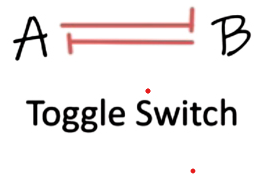
\includegraphics[width=20mm, scale=0.5]{toggle_switch_logo.png}
\end{figure}

\subsubsection*{Process Topology Information:} This process builds 
the ODEs based on the circuit topology (input). As an example the above circuit 
will be represented as 
\begin{align}
  \frac{dA}{dt} &= G_A H^S (B, B_A^0, n_{BA}, \lambda^{-}_{BA}) - k_A A \notag \\
  \frac{dB}{dt} &= G_B H^S (A, A_B^0, n_{AB}, \lambda^{-}_{AB}) - k_B B \notag 
\end{align}
Where, $A$ and $B$ represents the concentration of the protein $A$ and $B$ as  
a function of time, $G_A$ and $G_B$ are the maximum production rate of $A$ and 
$B$. $k_A$ and $k_B$ are the innate degradatino rates of the the corresponding 
proteins, and $H^S$ is non-linear shifted Hill function defined as
\begin{align}
  H^S (B, B_A^0, n_{BA}, \lambda^{-}_{BA}) & \coloneqq  \lambda^{-}_{BA} +
   \frac{1 -\lambda^{-}_{BA}}{1 + \left( \frac{B}{B_A^0}\right)^{n_{BA}}}
   \notag
\end{align} 
$\lambda^{-}_{BA}$ is the maximum fold change of A caused by inhibitor B. 

When multiple regulators target a gene, the function form of the rate equations 
assumes that these regulators are independent and hence, the overall production
rate becomes the product of the innate production rate of the target genes and 
the shifted Hill functions for all the regulatory links. 

\subsubsection*{Estimatation of parameters:}
Ranges of the threshold values in the shifted Hill functions are estimated 
numerically to satisfy the ``half-functoinal'' rule. Most of the other 
parametes are preset and sampled via a random distribution (which is `uniform 
distribution' by default). All these parameters are stored in a `.prs' (parameter)
file (e.g. ``circuit.prs'').

\subsubsection*{Solve the ODE, Identify the stable steady states:} RACIPE 
repeats the simulates teh coupled ODEs numerically for each sampled parameter
set for a large number of random initial conditions (optional input to RACIPE) 
and the steady state solutions for eac parameter set are stored in the output 
solution files.  
% ************************************************************************* %
%                                 Case Study                                %
% ************************************************************************* %
\newpage
\section*{Case Study: Modelling cell-cycle of fission-yeast}
To show the effiency of Boolean and RACIPE based model, I have chosen an 
already well studied model of fission-yeast cell-cycle as a case-study. The 
goal here is to see how far we can go without any konwledge about the actual
parameter values of the network.

\subsection*{Introduction to the model:}
The full process of the cell-cycle consists of four stages: $G1 \rightarrow 
S \rightarrow G2 \rightarrow M$. Where 
\begin{itemize}
  \item G1: the cell grows in this phase 
  \item S: DNA synthesis and chromosome replication happens in this phase
  \item G2: Gap phase 
  \item M: Chromosomes are separated and the cell is divided in this phase
\end{itemize}
\begin{figure}[H]
  \centering
  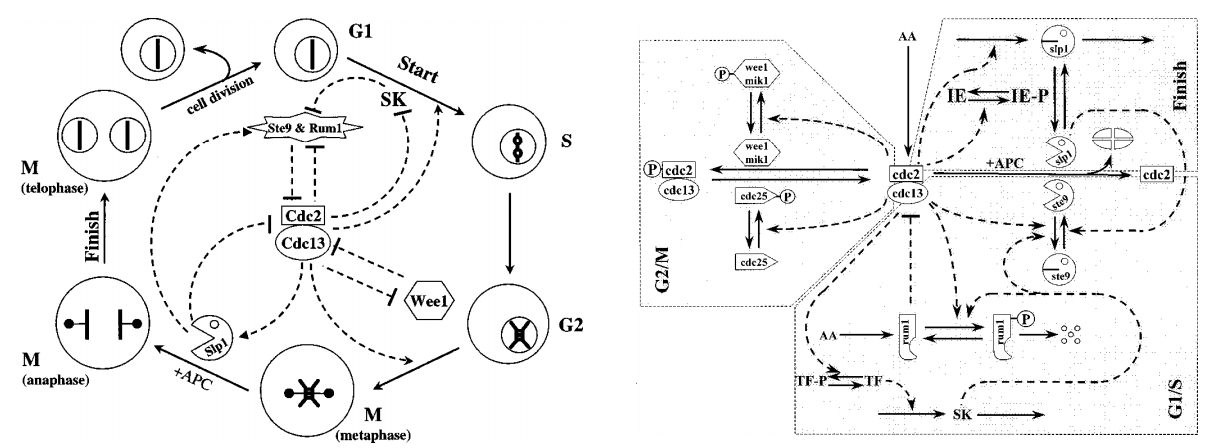
\includegraphics[width=\linewidth, scale=0.5]{cell_cycle_complicated.png}
\end{figure}
. \\
Figure 2: (Left) Outer cycle demonstrate the general phases of 
fission-yeast cell cycle and the inner network shows the raltionships among the 
principal molecular components. (Right) The wiring diagram of the cell-cycle 
engine emphasizing on the proteolysis of Cdc13 and phosphorylation of Cdc2 
subunit and their stoichiometric inhibition of the complex. \cite{math_model}
\newline \newline
the major role in fission-yeast cell-cycle is played by a cyclin dependent 
protine kinase complex Cdc2/Cdc13 with Tyr-15(also called MPF (M-phase promoting factor).
When Tyr-15 is unphosphorylated, the MPF complex reaches high activity (which we 
are going to represent as $Cdc2/Cdc13^*$ in the simplified model). This MPF complex
is inactive during G2 phase, when it is phosphorylated (represented as $Cdc2/Cdc13$).
The other members in the network are \textbf{positive regulators} of kinase Cdc2/Cdc13:
``Start'' (indicator of the mass/size of the cell), ``SK'' (Start Kinase), 
group of Cdk/ cyclin complexed and phosphatase Cdc25, and the \textbf{negative 
regulators}: ``Slp1'', ``Rum1'', ``Ste9'', and phosphatase ``PP''. This
simplified network is described in figure 3.
\begin{figure}[H]
  \centering
  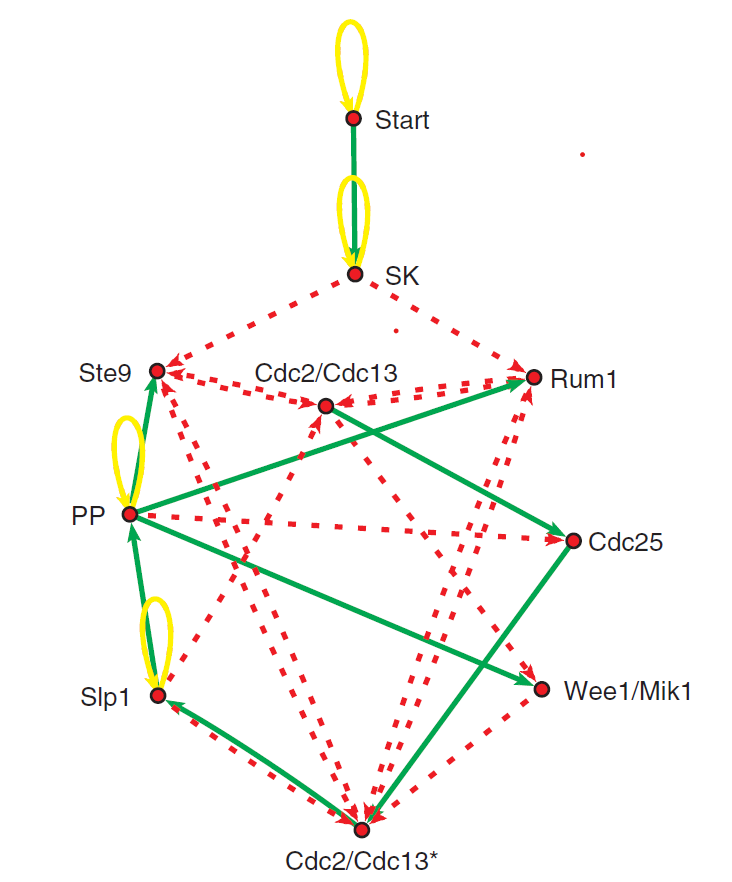
\includegraphics[width=\linewidth, scale=0.5]{cell_cycle_simple.png} \\
  \text{Figure 3: Simplied version of fission-yeast cell-cycle network \cite{boolean_model}}
\end{figure}
. \\
In the above network, the green edges denotes activation, the red dotted edges denote
inhibition, and the yellow loops denote self-degradation.
\subsubsection*{Discrete Method:}
The Biologically relevant starting condition for the network is All nodes OFF 
except Start, Ste9, Rum1, Wee1/Mik1. So, if we start the Boolean simulation of 
the network starting from the biolgical starting condition we get the time evolution
as shown in table 1.
\begin{figure}[H]
  \centering
  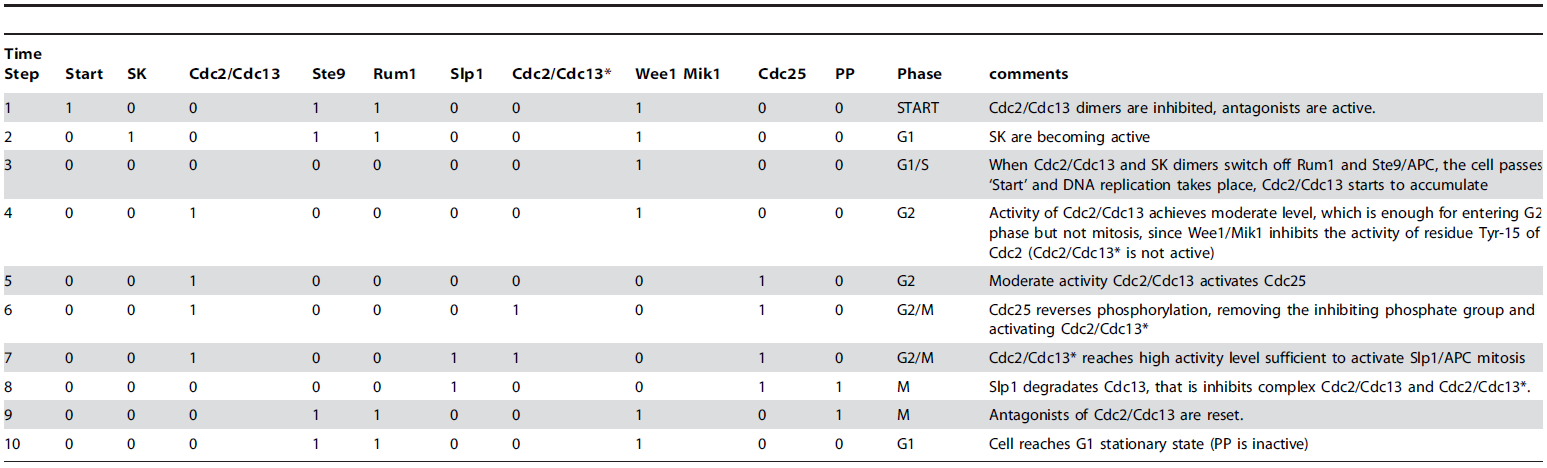
\includegraphics[width=\linewidth, scale=0.5]{bio_start_state_evo.png} \\
  \text{Table 1: Biologically relevant time evolution of the cell-cycle \cite{boolean_model}}
\end{figure}
.\\
the temporal evolution of the network surprisingly demonstrate some of the 
fundamental steps of cell-cycle, and the fun part is that the coputational 
requirement of this particular simulation is so small that we can even 
reproduce the result using just a pen and paper as well.

Then, if the Boolean model is simulated with all the $2^10 = 1024$ possible 
initial conditions, we can observe a bunch of stationary points emerging out 
of the simulation (preseneted in table 2). Surprisingly the largest attractor 
among those belongs to a fixed point attracting $73\%$ of all network states 
and that state belongs to biological \textbf{G1 phase}.
\begin{figure}[H]
  \centering
  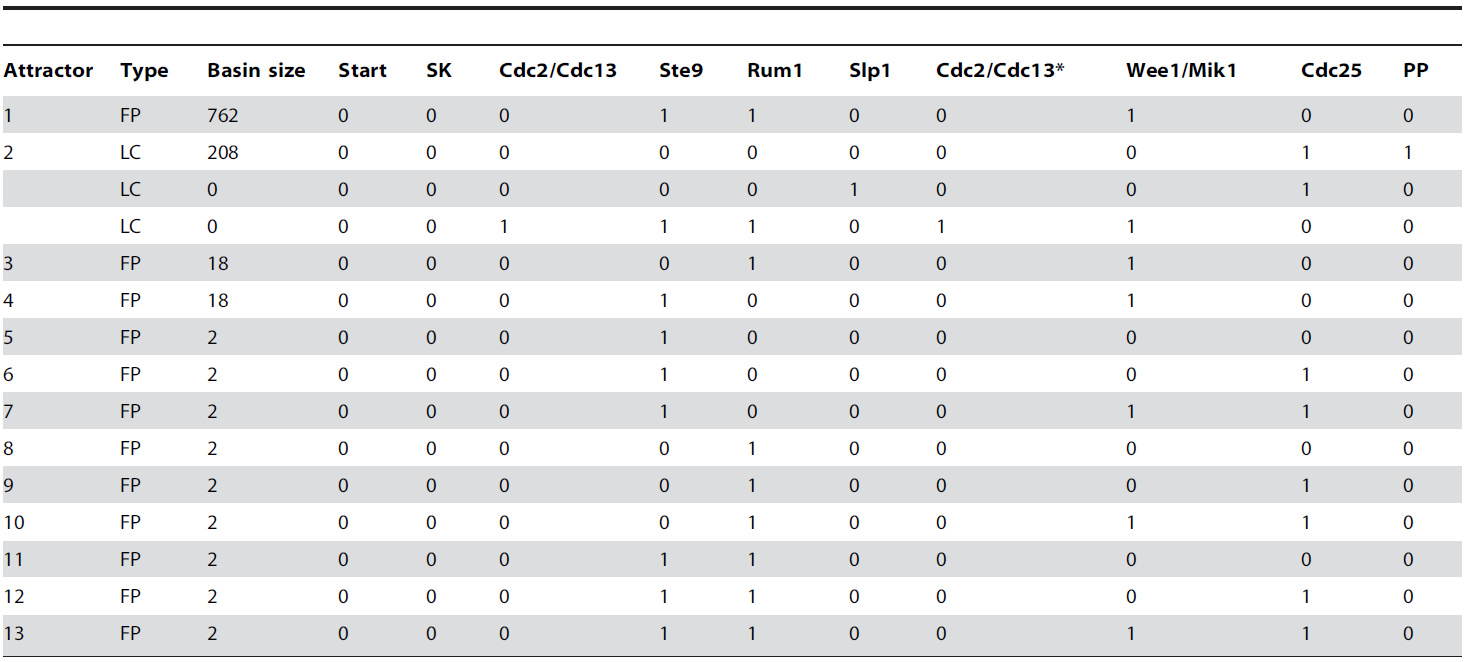
\includegraphics[width=\linewidth, scale=0.5]{fixed_point_bool.png} \\
  \text{Table 2: All attractors found in the Boolean simulation \cite{boolean_model}}
\end{figure}

\subsubsection*{Continuous Method:} 
Although the Boolean simulation gave us some quite useful information about
the network, it cannot possible encompass all about the the network because 
of its gross partining of states into HIGH and LOW and discrete time evolution,
which \textit{does not} happen in reality. Besides, ther are only 1024 inital 
conditions possible in the discrete model, which does not represents all the 
solution space.

To deal with the above issues, I have tried to use RACIPE simulations to model 
this network. But, there is a fundamental design clash of using RACIPE to 
simulate this model, because RACIPE was primarily built to show the robust 
steady states shown by gene regulatory networks where our we should expect to 
see primarily cycles in our fission-yeast cell-cycle network due to its 
biological function. So, to deal with these issues, I have tried to merge some 
of my own codes along with RACIPE in order to gain some ideas of the cycles 
seen in this network. 
\newline \newline 
Our first task is to get hints about oscillations from the RACIPE ouputs. For,
that we can simply plot the different stability states shown by the RACIPE 
solution files. From figure 4, we can see that around 8800 out of 10000 parameter
sets have given rise to mono-stable and bi-stable steady state solutions, where 
as rest of the 1000 parameters have given rise to apprantly `decastable solutions', 
which might sound absurd. But, what we are just seeing is a design choice present 
in RACIPE. First of all, the $10^{th}$ columns shows solutions which are decastable 
or higher. But, as we can observe that multistable solutions beyond tristability is 
statistically insignificant, possibility of presence of decastable solutions are 
almost none. So, what is happening here is that, when the parameter sets give rise 
to an oscillating pattern and not a steady state, the RACIPE simulation keeps getting 
last value of its numerical simulation in different conditions for all the 
randomly sampled inital conditions, and ends up deciding that the solution state 
is a higher-order multistable state and puts in the 10th column. So, basically that 
presence of 1000 parameter sets giving rise of decastable solutions is actually saying 
that 1000 out 10000 sampled parameters showed oscillations, which was expected 
from a cell-cycle network.
\begin{figure}[H]
  \centering
  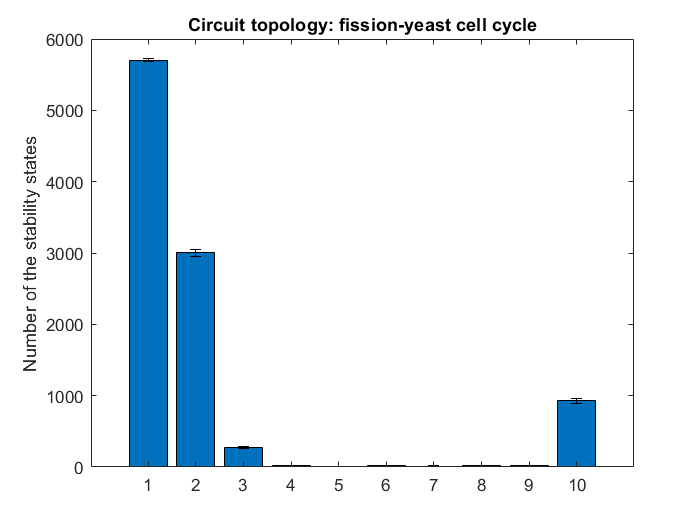
\includegraphics[width=100mm, scale=0.5]{stability_states.png} \\
  \text{Figure 4: Multistability solutions from RACIPE simulation} \\
  \text{X-axis $\rightarrow$ 1: Monostable solutions, 2: Bistable solutions, ...}
\end{figure}
.\\

To test my hypothesis, I wrote down a MATLAB program to extract the parameter 
sets sampled by RACIPE (present in the `.prs' file) giving rise to the 
``decastable'' solutions and simulate in the same manner via coupled ODEs 
using shifted Hill equations and plotted the dynamics of those network for 
random 10 (close to biologically relevant) initial conditions. I plotted 
the dynamics of the circuit w.r.t time for 4 random parameter sets and found that 
indeed most of those parameter sets gave rise to oscillating cycles as visible 
in figure 5 plots.  

\begin{figure}[H]
  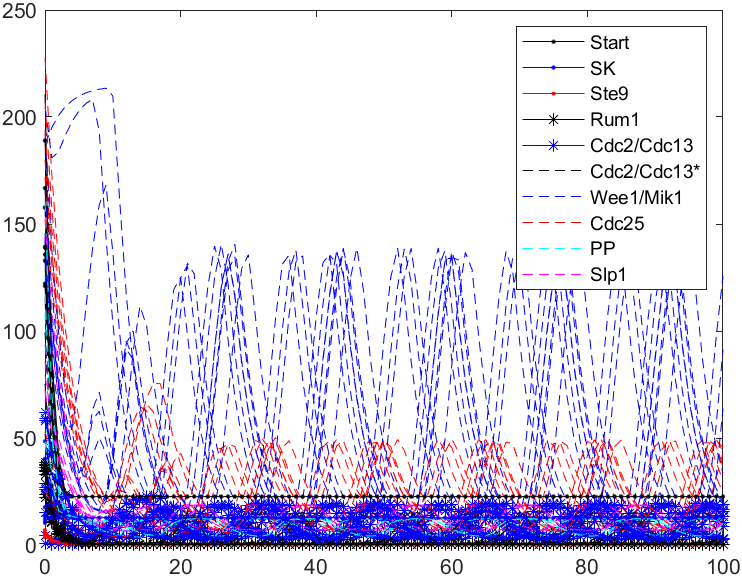
\includegraphics[width=60mm, scale=0.5]{dynamics1.png}
  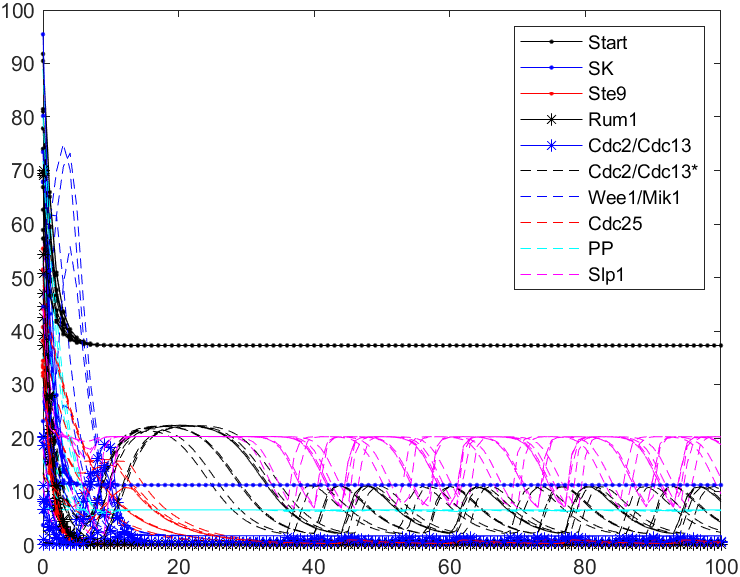
\includegraphics[width=60mm, scale=0.5]{dynamics2.png} 
  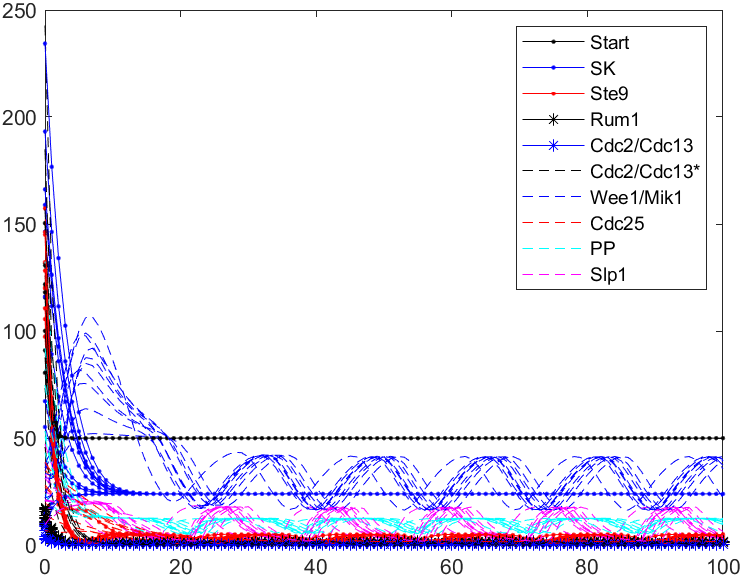
\includegraphics[width=60mm, scale=0.5]{dynamics3.png}
  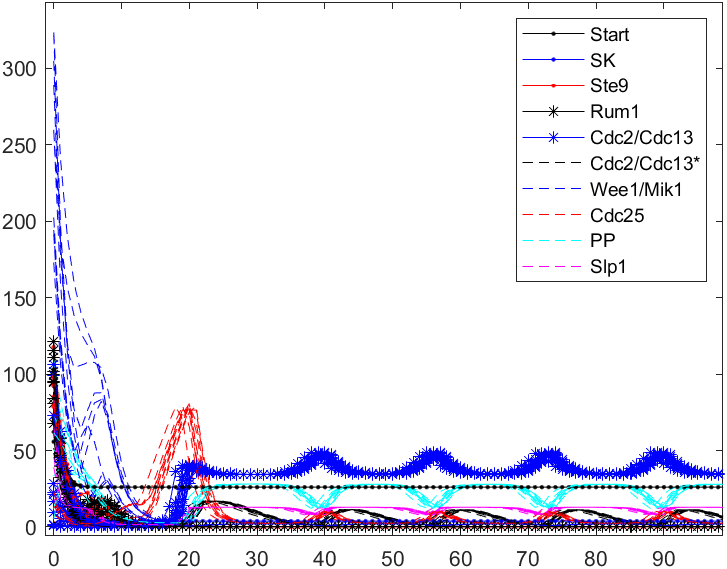
\includegraphics[width=60mm, scale=0.5]{dynamics5.png}
\end{figure}
.\\
Figure 5: Dynamics of the regulators of the network given the parameter sets 
generating decastable solutions in RACIPE. Y-axis is the concentration of the 
ten regulators and X-axis is time steps.
\newline \newline 
Next, I tried to observe the RACIPE solutions and find any possible patterns 
and for that applied hierarchical clustering on that solution data and plotted 
the histogram given in figure 6.
\begin{figure}[H]
  \centering
  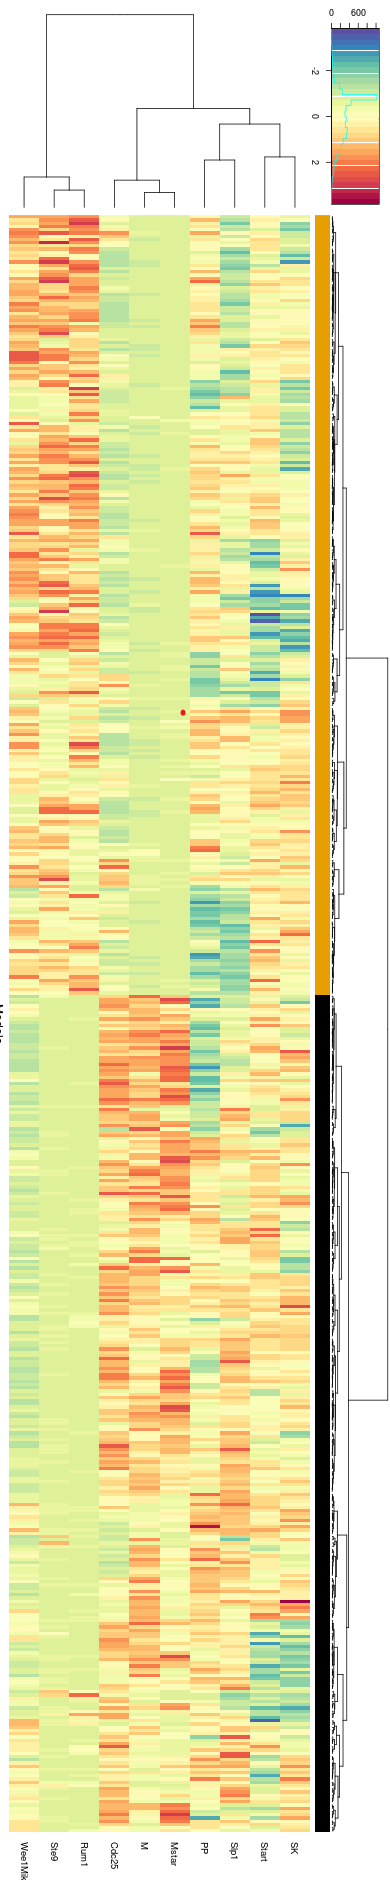
\includegraphics[width=38mm, scale=0.5]{hierarchical_clustering.png} \\
  \text{Figure 6: Hierarchical clustering of RACIPE simulation data} \\
  \text{M $\coloneqq Cdc2/Cdc13$, M-star $\coloneqq Cdc2/Cdc13^*$}
\end{figure}
\newpage
As I could not find any clear clustering present in the solution, I wrote MATLAB 
code to individally check each solutions of the monostable and bistable conditions
and ploted how many parameter-sets gave rise to each of the solution-state (representing 
attractors of the systems). I have plotted the statistically significant states 
that are often found in the vast solution spce of the RACIPE solution due to its 
highly random nature of sampling inital conditions and parameter sets. So, for 
that purpose, I have first converted the solutions give in RACIPE files 
(I performed three independent RACIPE simulations to attain statistically 
significant results) from 
log2 scale to normal scale, performed G/K normalization and Z-normalization on 
the data, to make it more presentable, and then kept tab on each and every solution
that fall in one of the solution-state bucket created by my code. I plotted 
the most frequently found mono and bi-stable steady state solutions as evident 
in figure 7. In these plots, we found all the attractors found in Boolean simulation
and many more. Although, the G1 biological state condition is not the most frequent 
state in the RACIPE simulations, it is still there and statistically much more significant 
than around thousands others attractors present in the RACIPE simulation.
\begin{figure}[H]
  \centering
  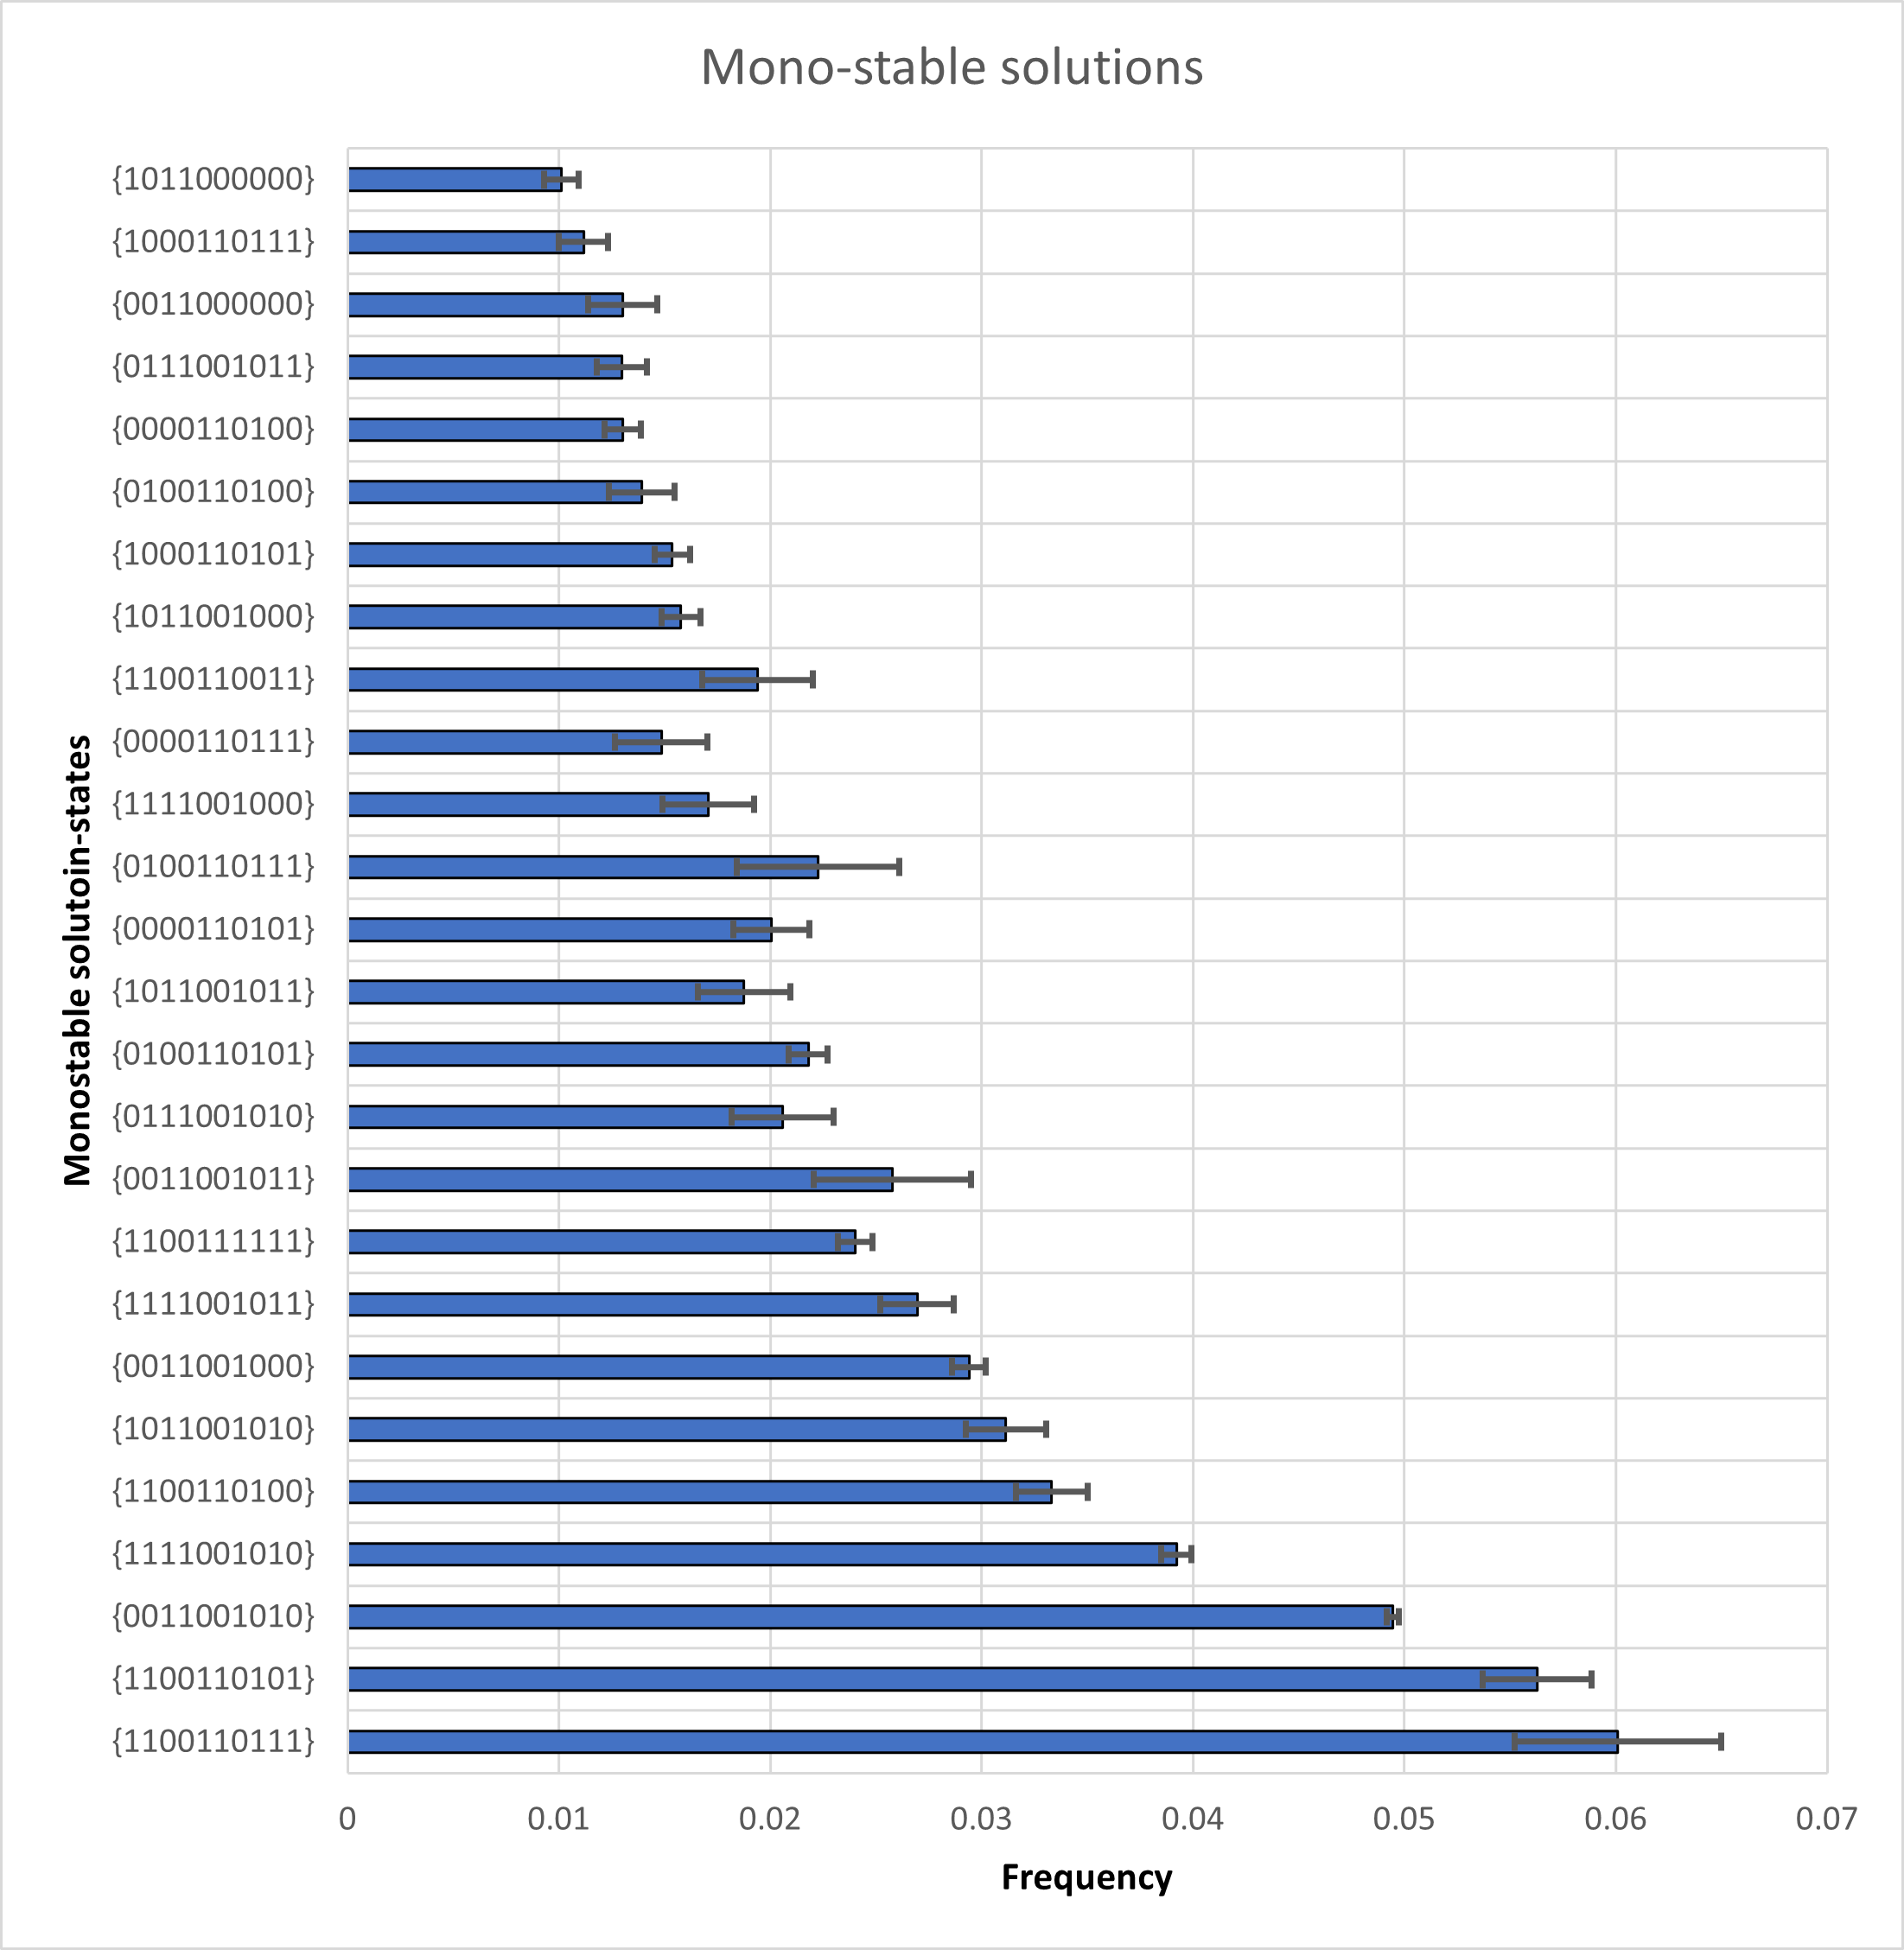
\includegraphics[width=110mm, scale=0.5]{monostable-freq.png}
\end{figure}
\begin{figure}[H]
  \centering
  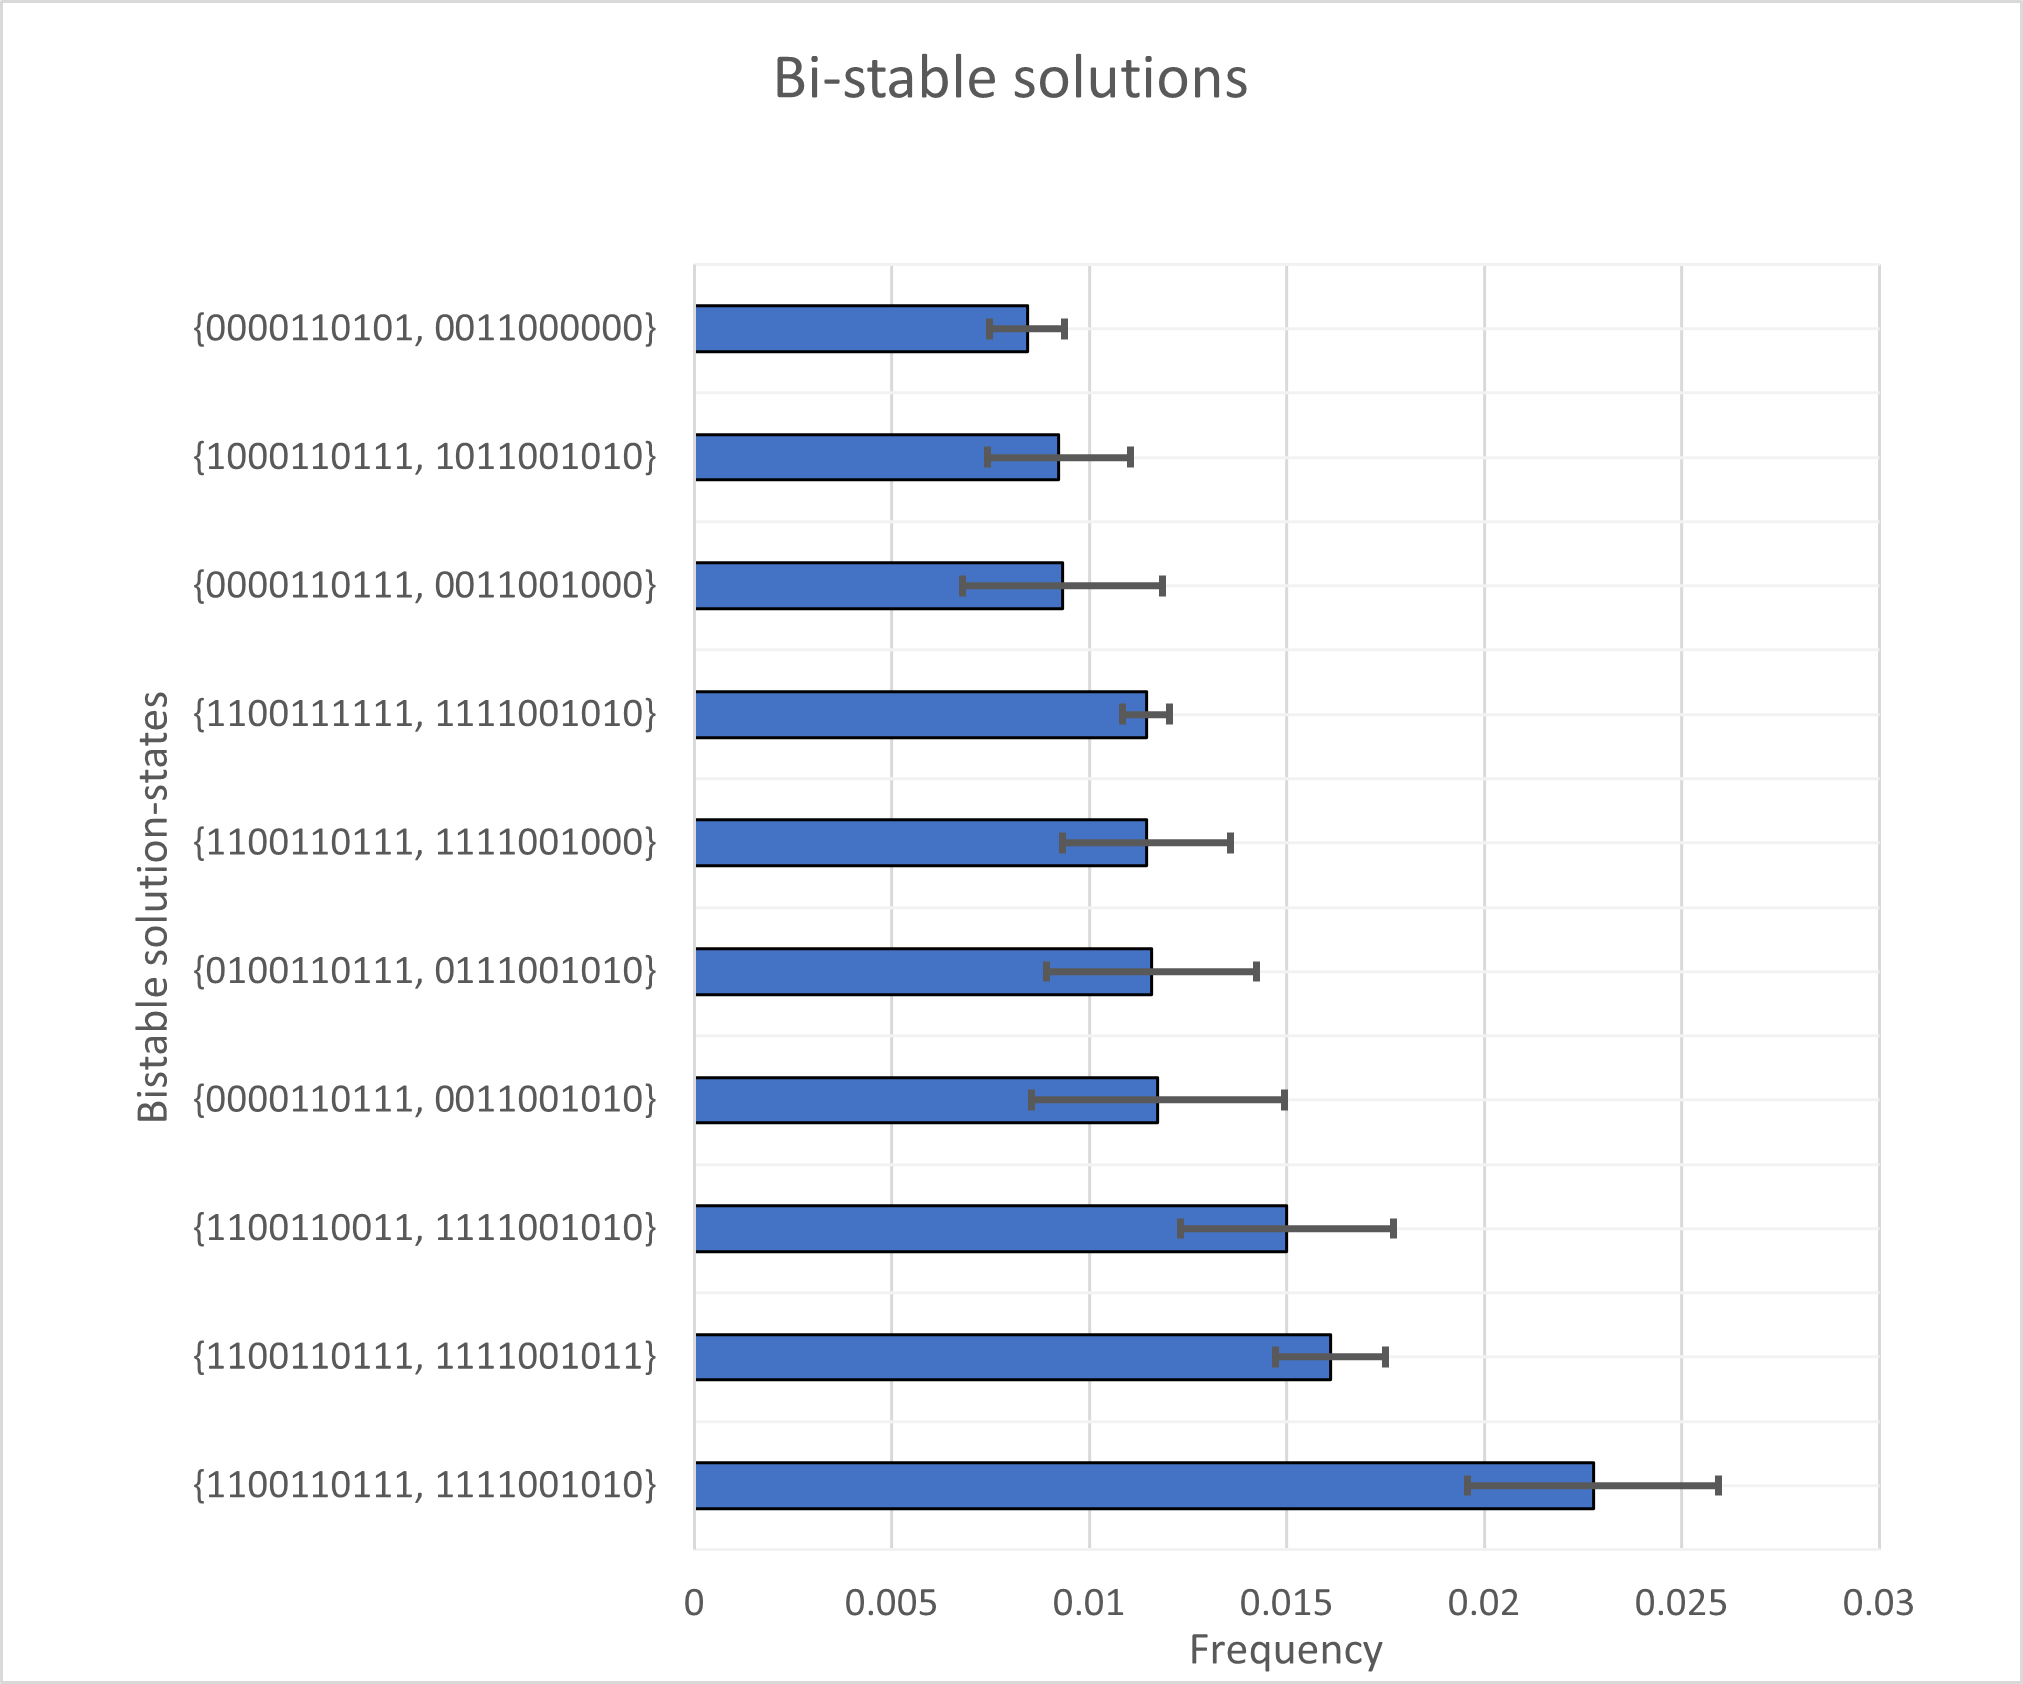
\includegraphics[width=110mm, scale=0.5]{bistable-freq.png}
  \text{Figure 7: Attractors of the cell-cycle network} \\
\end{figure}
. \\
The naming convention of the above states are as follows: $1$ denotes HIGH, 
and $0$ denotes LOW state. And those ten consecutive sequences of ones and zeros
basically shows the high/low concentration of $Start, SK, Ste9, Cdc2/Cdc13,$ 
$Cdc2/Cdc13^*, Wee1/Mik1, Cdc25, PP, \mbox{ and } Slp1$ in that exact order.

\section*{Shortcomings of these models and Future work:}
Despite showing such detailed information of the fissoin yeast cell-cycle network,
there is some inherent shortcomings of these methods and also some lack of 
expertise from my side as well. 

First, I need to perform some more analysis of the cycles shown by the decastable 
parameter states to see how close those oscillations are to the biologically 
seen oscillation of those regulators in the cell-cycle. 

Next, I need to do some more literature review to find the biological 
significance of those monostable and bistable steady-state solutions.

Atlast, although Boolean, despite being such computatoinally effienct method was
capable of providing stark amount of details of this cell-cycle network, 
RACIPE was a bad choice of software for a gene regulatory network whose primary 
job is to maintain an oscillation and not converging to some stable states. This 
required me to write a lot of additional codes to tackle with some of those 
inherent RACIPE specific problem, which is not ideally expected from RACIPE, 
which is already computationally expensive.
% ************************************************************************* %
%                                  THE END                                  %
% ************************************************************************* %
% ************************************************************************* %
%                                References                                 %
% ************************************************************************* %
\bibliography{citation} 
\bibliographystyle{abbrv}
% ************************************************************************* %  
\end{document} 